\documentclass{standalone}
\usepackage{tikz}
\usetikzlibrary{patterns, positioning}


\begin{document}
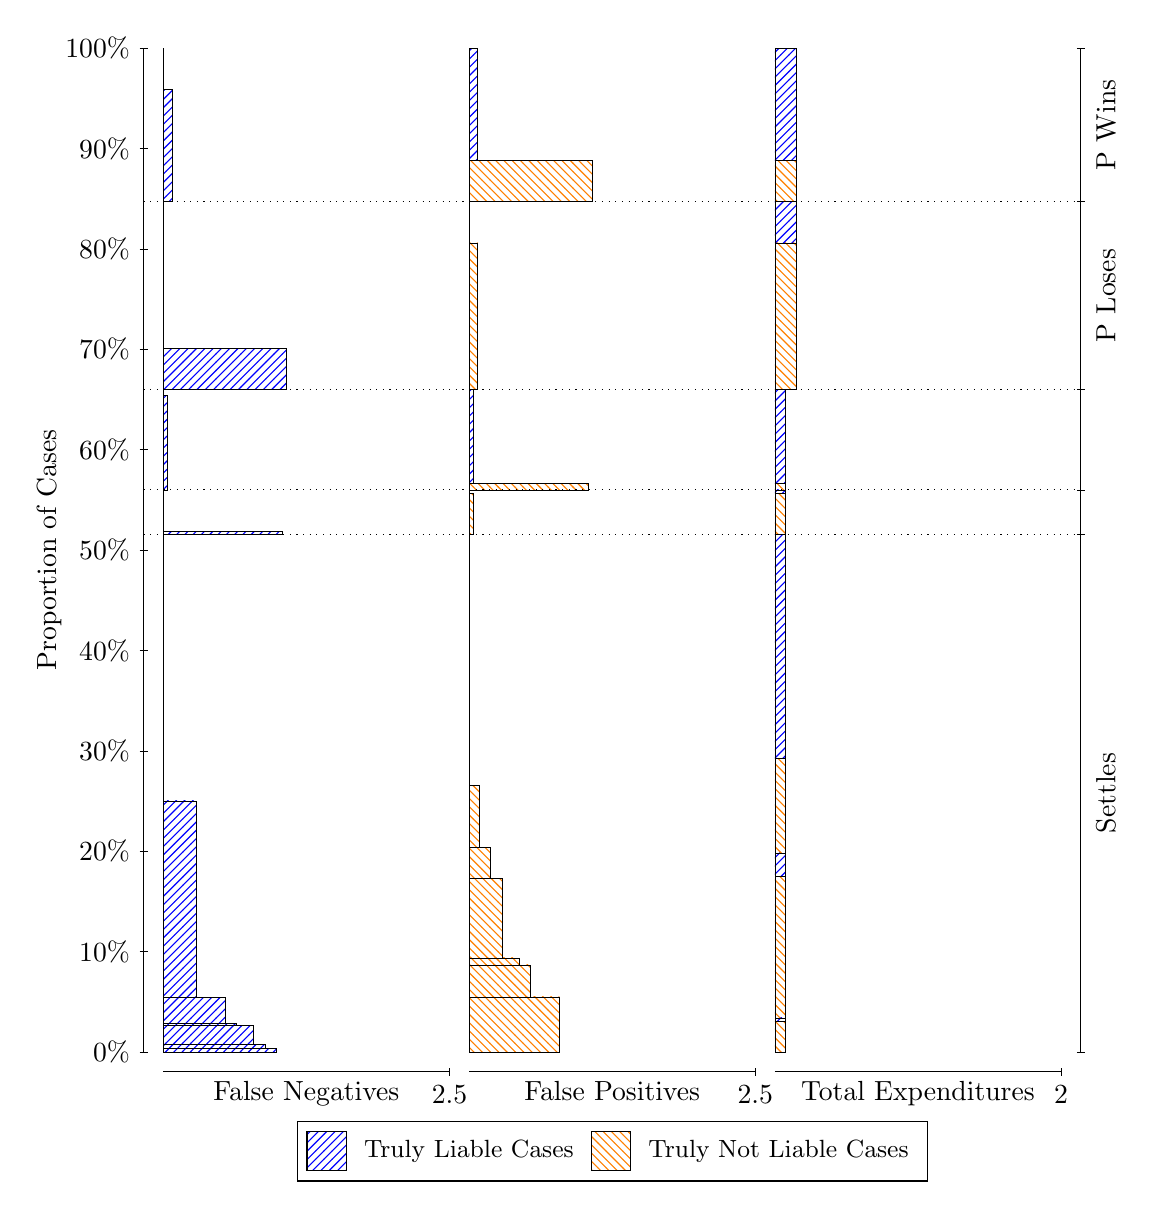
\begin{tikzpicture}
\draw[black, very thin] (1.5,1.75) -- (1.5,14.5);
\node[rotate=90, text=black, anchor=center] at (0.3, 8.125) {Proportion of Cases};
\draw[black, very thin] (1.45,1.75) -- (1.55,1.75);
\node[text=black, anchor=east] at (1.45, 1.75) {0\%};
\draw[black, very thin] (1.45,3.025) -- (1.55,3.025);
\node[text=black, anchor=east] at (1.45, 3.025) {10\%};
\draw[black, very thin] (1.45,4.3) -- (1.55,4.3);
\node[text=black, anchor=east] at (1.45, 4.3) {20\%};
\draw[black, very thin] (1.45,5.575) -- (1.55,5.575);
\node[text=black, anchor=east] at (1.45, 5.575) {30\%};
\draw[black, very thin] (1.45,6.85) -- (1.55,6.85);
\node[text=black, anchor=east] at (1.45, 6.85) {40\%};
\draw[black, very thin] (1.45,8.125) -- (1.55,8.125);
\node[text=black, anchor=east] at (1.45, 8.125) {50\%};
\draw[black, very thin] (1.45,9.4) -- (1.55,9.4);
\node[text=black, anchor=east] at (1.45, 9.4) {60\%};
\draw[black, very thin] (1.45,10.675) -- (1.55,10.675);
\node[text=black, anchor=east] at (1.45, 10.675) {70\%};
\draw[black, very thin] (1.45,11.95) -- (1.55,11.95);
\node[text=black, anchor=east] at (1.45, 11.95) {80\%};
\draw[black, very thin] (1.45,13.225) -- (1.55,13.225);
\node[text=black, anchor=east] at (1.45, 13.225) {90\%};
\draw[black, very thin] (1.45,14.5) -- (1.55,14.5);
\node[text=black, anchor=east] at (1.45, 14.5) {100\%};

\draw[black, very thin] (13.4,1.75) -- (13.4,14.5);
\draw[black, very thin] (13.35,1.75) -- (13.45,1.75);
\node[anchor=west] at (13.35, 1.75) {};
\draw[black, very thin] (13.35,8.3248) -- (13.45,8.3248);
\node[anchor=west] at (13.35, 8.3248) {};
\draw[black, very thin] (13.35,8.8882) -- (13.45,8.8882);
\node[anchor=west] at (13.35, 8.8882) {};
\draw[black, very thin] (13.35,10.163) -- (13.45,10.163);
\node[anchor=west] at (13.35, 10.163) {};
\draw[black, very thin] (13.35,12.549) -- (13.45,12.549);
\node[anchor=west] at (13.35, 12.549) {};
\draw[black, very thin] (13.35,14.5) -- (13.45,14.5);
\node[anchor=west] at (13.35, 14.5) {};

\draw[black, very thin, pattern color=blue, pattern=north east lines] (1.75,1.75) rectangle (3.1852,1.7996);
\draw[black, very thin, pattern color=blue, pattern=north east lines] (1.75,1.7996) rectangle (3.0398,1.8445);
\draw[black, very thin, pattern color=blue, pattern=north east lines] (1.75,1.8445) rectangle (2.8945,2.0885);
\draw[black, very thin, pattern color=blue, pattern=north east lines] (1.75,2.0885) rectangle (2.6765,2.1172);
\draw[black, very thin, pattern color=blue, pattern=north east lines] (1.75,2.1172) rectangle (2.5312,2.4421);
\draw[black, very thin, pattern color=blue, pattern=north east lines] (1.75,2.4421) rectangle (2.1678,4.9387);
\draw[black, very thin, pattern color=orange, pattern=north west lines] (1.75,4.9387) rectangle (1.75,8.3248);
\draw[black, very thin, pattern color=blue, pattern=north east lines] (1.75,8.3248) rectangle (3.2578,8.3646);
\draw[black, very thin, pattern color=orange, pattern=north west lines] (1.75,8.3646) rectangle (1.75,8.8882);
\draw[black, very thin, pattern color=blue, pattern=north east lines] (1.75,8.8882) rectangle (1.8045,10.084);
\draw[black, very thin, pattern color=orange, pattern=north west lines] (1.75,10.084) rectangle (1.75,10.163);
\draw[black, very thin, pattern color=blue, pattern=north east lines] (1.75,10.163) rectangle (3.3123,10.686);
\draw[black, very thin, pattern color=orange, pattern=north west lines] (1.75,10.686) rectangle (1.75,12.549);
\draw[black, very thin, pattern color=blue, pattern=north east lines] (1.75,12.549) rectangle (1.859,13.976);
\draw[black, very thin, pattern color=orange, pattern=north west lines] (1.75,13.976) rectangle (1.75,14.5);
\draw[black, very thin, pattern color=orange, pattern=north west lines] (5.6333,1.75) rectangle (6.7778,2.4493);
\draw[black, very thin, pattern color=orange, pattern=north west lines] (5.6333,2.4493) rectangle (6.4145,2.8548);
\draw[black, very thin, pattern color=orange, pattern=north west lines] (5.6333,2.8548) rectangle (6.2692,2.9462);
\draw[black, very thin, pattern color=orange, pattern=north west lines] (5.6333,2.9462) rectangle (6.0512,3.9585);
\draw[black, very thin, pattern color=orange, pattern=north west lines] (5.6333,3.9585) rectangle (5.9058,4.3452);
\draw[black, very thin, pattern color=orange, pattern=north west lines] (5.6333,4.3452) rectangle (5.7605,5.1361);
\draw[black, very thin, pattern color=blue, pattern=north east lines] (5.6333,5.1361) rectangle (5.6333,8.3248);
\draw[black, very thin, pattern color=orange, pattern=north west lines] (5.6333,8.3248) rectangle (5.6878,8.8483);
\draw[black, very thin, pattern color=blue, pattern=north east lines] (5.6333,8.8483) rectangle (5.6333,8.8882);
\draw[black, very thin, pattern color=orange, pattern=north west lines] (5.6333,8.8882) rectangle (7.1412,8.9673);
\draw[black, very thin, pattern color=blue, pattern=north east lines] (5.6333,8.9673) rectangle (5.6878,10.163);
\draw[black, very thin, pattern color=orange, pattern=north west lines] (5.6333,10.163) rectangle (5.7423,12.026);
\draw[black, very thin, pattern color=blue, pattern=north east lines] (5.6333,12.026) rectangle (5.6333,12.549);
\draw[black, very thin, pattern color=orange, pattern=north west lines] (5.6333,12.549) rectangle (7.1957,13.073);
\draw[black, very thin, pattern color=blue, pattern=north east lines] (5.6333,13.073) rectangle (5.7423,14.5);
\draw[black, very thin, pattern color=orange, pattern=north west lines] (9.5167,1.75) rectangle (9.6529,2.1367);
\draw[black, very thin, pattern color=blue, pattern=north east lines] (9.5167,2.1367) rectangle (9.6529,2.1816);
\draw[black, very thin, pattern color=orange, pattern=north west lines] (9.5167,2.1816) rectangle (9.6529,3.9848);
\draw[black, very thin, pattern color=blue, pattern=north east lines] (9.5167,3.9848) rectangle (9.6529,4.2784);
\draw[black, very thin, pattern color=orange, pattern=north west lines] (9.5167,4.2784) rectangle (9.6529,5.4746);
\draw[black, very thin, pattern color=blue, pattern=north east lines] (9.5167,5.4746) rectangle (9.6529,8.3248);
\draw[black, very thin, pattern color=orange, pattern=north west lines] (9.5167,8.3248) rectangle (9.6529,8.8483);
\draw[black, very thin, pattern color=blue, pattern=north east lines] (9.5167,8.8483) rectangle (9.6529,8.8882);
\draw[black, very thin, pattern color=orange, pattern=north west lines] (9.5167,8.8882) rectangle (9.6529,8.9673);
\draw[black, very thin, pattern color=blue, pattern=north east lines] (9.5167,8.9673) rectangle (9.6529,10.163);
\draw[black, very thin, pattern color=orange, pattern=north west lines] (9.5167,10.163) rectangle (9.7892,12.026);
\draw[black, very thin, pattern color=blue, pattern=north east lines] (9.5167,12.026) rectangle (9.7892,12.549);
\draw[black, very thin, pattern color=orange, pattern=north west lines] (9.5167,12.549) rectangle (9.7892,13.073);
\draw[black, very thin, pattern color=blue, pattern=north east lines] (9.5167,13.073) rectangle (9.7892,14.5);
\draw[black, dotted] (1.5,8.3248) -- (13.4,8.3248);
\draw[black, dotted] (1.5,8.8882) -- (13.4,8.8882);
\draw[black, dotted] (1.5,10.163) -- (13.4,10.163);
\draw[black, dotted] (1.5,12.549) -- (13.4,12.549);
\draw[black, very thin] (1.75,1.5) -- (5.3833,1.5);
\node[text=black, anchor=north] at (3.5667, 1.5) {False Negatives};
\draw[black, very thin] (5.3833,1.45) -- (5.3833,1.55);
\node[text=black, anchor=north] at (5.3833, 1.45) {2.5};

\draw[black, very thin] (5.6333,1.5) -- (9.2667,1.5);
\node[text=black, anchor=north] at (7.45, 1.5) {False Positives};
\draw[black, very thin] (9.2667,1.45) -- (9.2667,1.55);
\node[text=black, anchor=north] at (9.2667, 1.45) {2.5};

\draw[black, very thin] (9.5167,1.5) -- (13.15,1.5);
\node[text=black, anchor=north] at (11.333, 1.5) {Total Expenditures};
\draw[black, very thin] (13.15,1.45) -- (13.15,1.55);
\node[text=black, anchor=north] at (13.15, 1.45) {2};

\node[text=black, centered, rotate=90] at (13.72, 5.0374) {Settles};


\node[text=black, centered, rotate=90] at (13.72, 11.356) {P Loses};
\node[text=black, centered, rotate=90] at (13.72, 13.525) {P Wins};

\draw (7.449999999999999,1.5) node[draw=none] (baseCoordinate) {};
\begin{scope}[align=center]
        \matrix[scale=0.5, draw=black, below=0.5cm of baseCoordinate, nodes={draw}, column sep=0.1cm]{
            \node[rectangle, draw, minimum width=0.5cm, minimum height=0.5cm, pattern color=blue, pattern=north east lines] {}; &
            \node[draw=none, font=\small, text=black] (B) {Truly Liable Cases}; &
            \node[rectangle, draw, minimum width=0.5cm, minimum height=0.5cm, pattern color=orange, pattern=north west lines] {}; &
            \node[draw=none, font=\small, text=black] (B) {Truly Not Liable Cases}; \\
            };
\end{scope}

\end{tikzpicture}
\end{document}